\documentclass{article}
\usepackage{ listings} 
\usepackage{amsmath}
\usepackage{float} 
\usepackage{graphicx}
\usepackage{subcaption}
\usepackage{geometry}
\usepackage{amsthm}
\usepackage{amssymb}

\begin{document}
\title{Solution to Homework 2}
\author{Shoeb Mohammed and Zhuo Chen}
\maketitle

\newcommand{\QEDA}{\hfill\ensuremath{\blacksquare}}
\newcommand{\QEDB}{\hfill\ensuremath{\square}}

\section{Gradient and Hessian of $NLL(\theta)$ for logistic regression}
\subsection{}
Given
\begin{equation}
  \label{eq:1.1}
  g(z) = \frac{1}{1+e^{-z}}
\end{equation}

\begin{proof}
\begin{equation}
  \label{eq:1.2}
  \frac{\partial g(z)}{\partial z} = \frac{(1+e^{-z}).0 + e^{-z}}{(1+e^{-z})^2} = \frac{e^{-z}}{(1+e^{-z})^2} = g(z)(1-g(z))
\end{equation}
\end{proof}
\subsection{}

\newcommand{\HthetaXi}{h_\theta(x_i)}

For logistic regression, negative log likelihood is
\begin{equation}
  \label{eq:1.3}
  NLL(\theta)  = - \sum_{i=1}^{m} \left( y_i log(\HthetaXi) + (1-y_i)log(1-\HthetaXi) \right) \text{ where } \HthetaXi = g(\theta^Tx^i)
\end{equation}

\begin{proof}
Using equation~\ref{eq:1.2} and chain rule for differentiation we have
\begin{equation}
  \label{eq:1.4}
  \begin{split}
  NLL(\theta)  &= - \sum_{i=1}^{m} \left( \frac{y_i}{\HthetaXi}\HthetaXi(1-\HthetaXi)\frac{\partial \theta^T x^i}{\partial \theta} 
                                         - \frac{(1-y_i)}{(1-\HthetaXi)}\HthetaXi(1-\HthetaXi)\frac{\partial \theta^T x^i}{\partial \theta} \right) \\
               &= - \sum_{i=1}^{m} \left( y_i(1-\HthetaXi) - (1-y_i)\HthetaXi\right) x_i \text{ because } \frac{\partial}{\partial \theta} \theta^T x^i = x^i \\
               &=   \sum_{i=1}^{m} \left(\HthetaXi - y_i\right)
  \end{split}
\end{equation}
\end{proof}


\subsection{}
Given

\begin{equation}
  \label{eq:1.5}
  \begin{split}
  H = X^T S X  \text{ where } &S = diag(\mu_1 \hdots \mu_m) \\
                              &\mu_i = \HthetaXi(1-\HthetaXi) \text{ for } i = 1 \hdots m \\
                              &\text{and } 0 < \mu_i < 1 \text{ for } i = 1 \hdots m
  \end{split}
\end{equation}

\begin{proof}
For any vector $u \neq 0$ we have,
\begin{equation}
  \label{eq:1.6}
  \begin{split}
    u^T H u  &= u^T (X^T S X) u \\
             &= (Xu)^T S (Xu)  \\
             &= v^T S v \text{ where } v = [v_1 \hdots v_m]^T = Xu \neq 0 \text{ since $X$ is full rank} \\
             &= \sum_{i=1}^{m}v_i^2 \mu_i \\
             &> 0 \text{ since $\mu_i$  is positive and $v_i \neq 0$} 
  \end{split}
\end{equation}

Thus, $H$ is positive definite.
\end{proof}

\section{Regularizing logistic regression}
\begin{proof}
The maximal likehood and MAP estimates for $\theta$ are

\newcommand{\thetaMAP}{\theta_{MAP}}
\newcommand{\thetaMLE}{\theta_{MLE}}

\begin{equation}
  \label{eq:1.7}
  \begin{split}
  \thetaMLE &= argmax_{\theta}\prod_{i=1}^m P(y^{(i)} | x^{(i)} ; \theta) \\
  \thetaMAP &= argmax_{\theta}P(\theta)\prod_{i=1}^m P(y^{(i)} | x^{(i)} ; \theta) \text{ where } P(\theta) \sim N(0,\alpha^2I)
  \end{split}
\end{equation}

Equation~\ref{eq:1.7} can be rewritten using log likelihood $LL(\theta)$:
\begin{equation}
  \label{eq:1.8}
  \begin{split}
  \thetaMLE &= argmax_{\theta}LL(\theta) \text{ where } LL(\theta) = \sum_{i=1}^m log(P(y^{(i)} | x^{(i)} ; \theta)) \\
  \thetaMAP &= argmax_{\theta} log(P(\theta)) + LL(\theta) \\
            &= argmax_{\theta} K - \frac{d}{2\alpha^2}\theta^T\theta + LL(\theta) \text{ where $K$ is constant. This follows from $P(\theta) \sim N(0,\alpha^2I)$}\\
            &= argmax_{\theta}  LL(\theta) - \frac{d}{2\alpha^2}\Vert \theta \Vert_2^2
  \end{split}
\end{equation}


Now,
\begin{equation}
  \label{eq:1.9}
  \begin{split}
   LL(\thetaMAP) - \frac{d}{2\alpha^2}\Vert \thetaMAP \Vert_2^2 &\geq    LL(\thetaMLE) - \frac{d}{2\alpha^2}\Vert \thetaMLE \Vert_2^2 \text{\qquad from definition for $\thetaMAP$} \\
                                                                &\geq    LL(\thetaMAP) - \frac{d}{2\alpha^2}\Vert \thetaMLE \Vert_2^2 \text{\qquad from definition for $\thetaMLE$} \\
   \implies \frac{d}{2\alpha^2}\Vert \thetaMAP \Vert_2^2 &\leq \frac{d}{2\alpha^2}\Vert \thetaMLE \Vert_2^2 \\
   \implies \Vert \thetaMAP \Vert_2^2 &\leq \Vert \thetaMLE \Vert_2^2 \\
   \implies \Vert \thetaMAP \Vert_2 &\leq \Vert \thetaMLE \Vert_2 
  \end{split}
\end{equation}
\end{proof}
\section{Implementing logistic regression}
\subsection{Part A}
\paragraph{Implementing logistic regression : the sigmoid function\\}
------\\
Implemented \verb|sigmoid| method in \verb|utils.py|.
\begin{tiny}
\begin{lstlisting}
def sigmoid (z):
    sig = np.zeros(z.shape)
    # Your code here
    sig = 1/(1+np.exp(-1*z))
    # End your ode
    return sig

\end{lstlisting}
\end{tiny}

\paragraph{Cost function and gradient of logistic regression\\}
------\\
Implemented  \verb|loss| and  \verb|grad_loss| methods in the  \verb|LogisticRegressor| class in   \verb|logistic_regressor.py|.
\begin{tiny}
\begin{lstlisting}
J=-1*np.sum(np.log(utils.sigmoid(np.dot(theta,X.T)))*y+np.log(1-utils.sigmoid(np.dot(theta,X.T)))*(1-y))/m

grad = np.dot((utils.sigmoid(np.dot(theta,X.T))-y),X)/m

\end{lstlisting}
\end{tiny}
\paragraph{Prediction using a logistic regression model\\}
------\\
Implemented \verb|predict| method in the  \verb|LogisticRegressor| class in \verb|logistic_regressor.py|.

\begin{tiny}
\begin{lstlisting}
y_pred = utils.bin_features(utils.sigmoid(np.dot(self.theta,X.T))-0.5)
\end{lstlisting}
\end{tiny}
Add code in \verb|ex1.py|.


\begin{tiny}
\begin{lstlisting}
pred_prob = utils.sigmoid(np.dot(log_reg1.theta,np.array([1,45,85]).T))

accuracy  = 1-float(np.sum(np.abs(predy-y)))/y.shape[0]
\end{lstlisting}
\end{tiny}

\paragraph{Result\\}
------\\
Run \verb|ex1.py| in the shell:
\begin{tiny}
\begin{lstlisting}
Plotting data with green circle indicating (y=1) examples and red circle indicating (y=0) examples ...
Loss on all-zeros theta vector (should be around 0.693) =  0.69314718056
Gradient of loss wrt all-zeros theta vector (should be around [-0.1, -12.01, -11.26]) =  [ -0.1        -12.00921659 -11.26284221]
Optimization terminated successfully.
         Current function value: 0.203498
         Iterations: 19
         Function evaluations: 20
         Gradient evaluations: 20
Theta found by fmin_bfgs:  [-25.16056945   0.20622963   0.20146073]
Final loss =  0.203497702351
For a student with 45 on exam 1 and 85 on exam 2, the probability of admission =  0.776246678481
Accuracy on the training set =  0.89
Theta found by sklearn:  [[-25.15293066   0.20616459   0.20140349]]
\end{lstlisting}
\end{tiny} 
\begin{figure}[H]\subcaptionbox{The training data\label{fig:1}}[.5\linewidth]{

	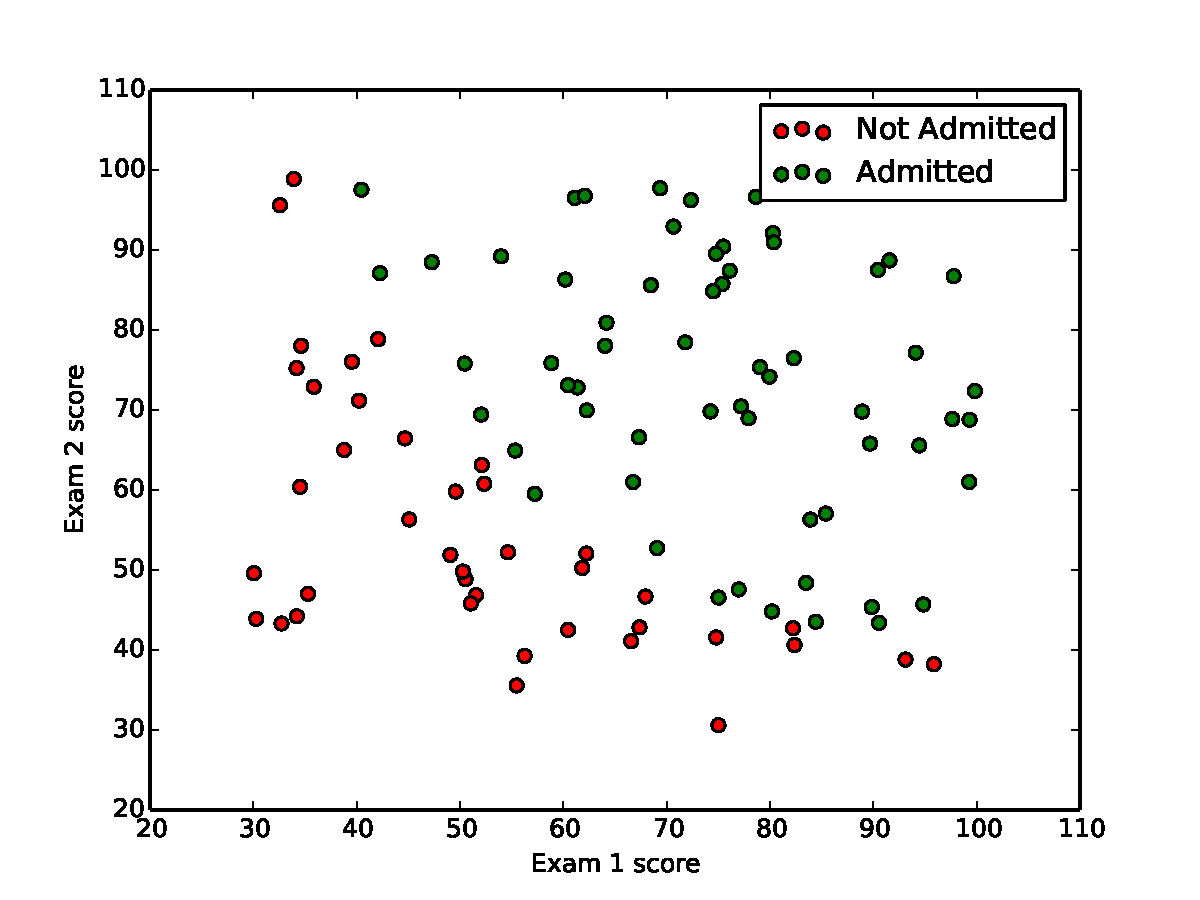
\includegraphics[width=7cm]{part1/fig1.pdf}

	}\subcaptionbox{The decision boundary\label{fig:2}}[.5\linewidth]{

	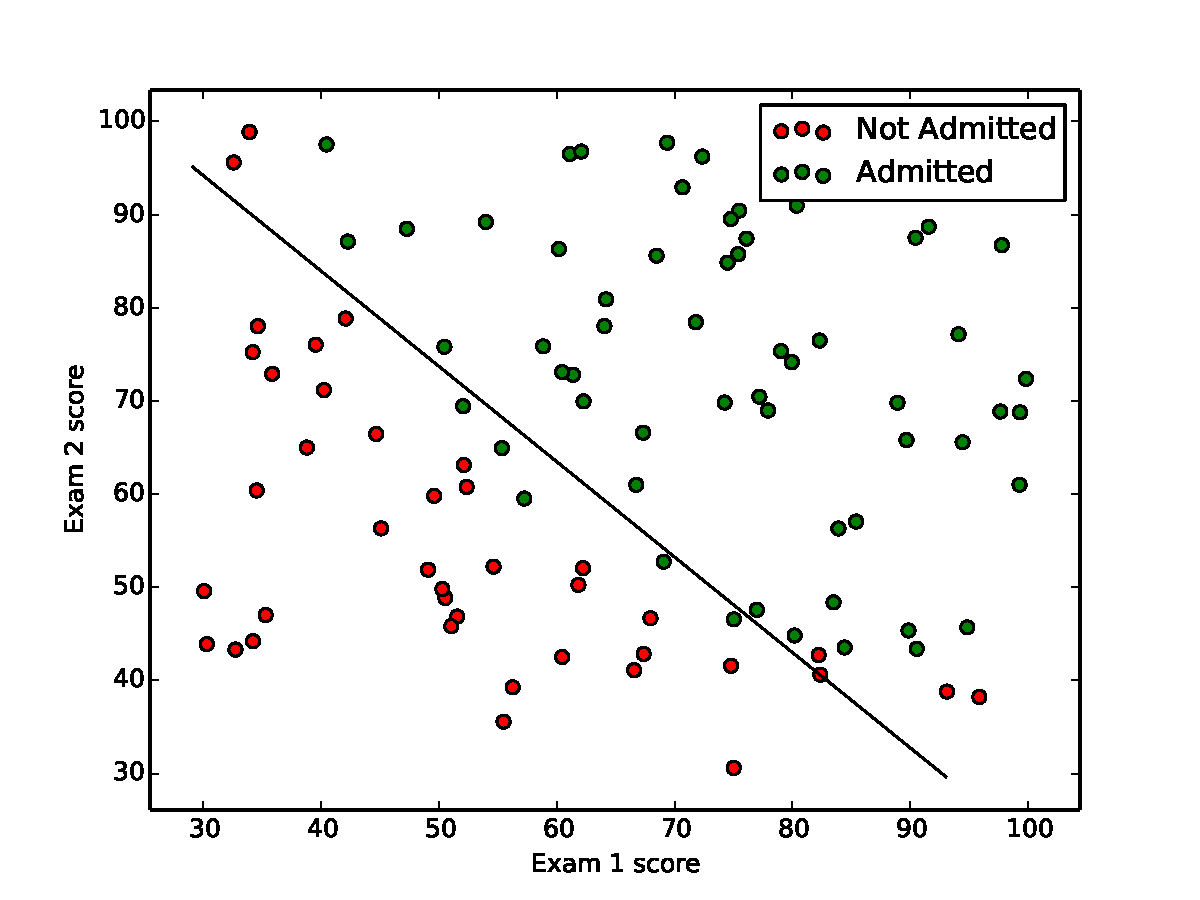
\includegraphics[width=7cm]{part1/fig2.pdf}

	}\caption{}
\end{figure}

All as expected.
\subsection{Part B}
\paragraph{Cost function and gradient for regularized logistic regression\\}
------\\
Implemented  \verb|loss| and  \verb|grad_loss| methods in the  \verb|RegLogisticRegressor| class in   \verb|logistic_regressor.py|.
\begin{tiny}
\begin{lstlisting} 
J=-1*np.sum(np.log(utils.sigmoid(np.dot(theta,X.T)))*y+np.log(1-utils.sigmoid(np.dot(theta,X.T)))*(1-y))/m
+reg*np.sum(theta[1:]**2)/2/m

grad = np.dot((utils.sigmoid(np.dot(theta,X.T))-y),X)/m

\end{lstlisting}
\end{tiny}
\paragraph{Prediction using the model\\}
------\\
Implemented \verb|predict| method in the  \verb|LogisticRegressor| class in \verb|logistic_regressor.py|.

\begin{tiny}
\begin{lstlisting}
y_pred = utils.bin_features(utils.sigmoid(np.dot(self.theta,X.T))-0.5)
\end{lstlisting}
\end{tiny}
Add code in \verb|ex1_reg.py|.


\begin{tiny}
\begin{lstlisting}
accuracy  = 1-float(np.sum(np.abs(predy-y)))/y.shape[0]
\end{lstlisting}
\end{tiny}
\paragraph{Varying λ\\}
------\\
Add code in \verb|ex1_reg.py|.
\begin{tiny}
\begin{lstlisting}
for reg in [0,1.0,100.0]:
...
\end{lstlisting}
\end{tiny}

\paragraph{Exploring L1 and L2 penalized logistic regression\\}
------\\
Add code in \verb|ex1_reg.py|.
\begin{tiny}
\begin{lstlisting}
for reg in [0.1,0.5,1.0,5.0,10.0]:
...
\end{lstlisting}
\end{tiny}
\paragraph{Result\\}
------\\
Run \verb|ex1_reg.py| in the shell:
\begin{tiny}
\begin{lstlisting}
Plotting data with green circle indicating (y=1) examples and red circle indicating (y=0) examples ...
Optimization terminated successfully.
         Current function value: 0.224569
         Iterations: 546
         Function evaluations: 547
         Gradient evaluations: 547
Theta found by fmin_bfgs:with reg = 0.0 [   35.10191556    44.11916104    69.27187135  -344.27909285  -198.23463329
  -184.2284154   -295.82041756  -621.7326024   -510.84919909  -328.31173228
  1094.70040538  1269.58583356  1757.74907248   900.93789211   436.58879589
   471.12031352  1236.23835236  1822.81976807  1929.66695582  1131.05273288
   463.79908073 -1142.11739081 -2020.95888645 -3463.39935641 -3484.5099411
 -3252.26696072 -1546.00910831  -510.41253513]
Final loss =  0.224568734073
Accuracy on the training set =  0.915254237288
Optimization terminated successfully.
         Current function value: 0.529003
         Iterations: 47
         Function evaluations: 48
         Gradient evaluations: 48
Theta found by fmin_bfgs:with reg = 1.0 [ 1.27268739  0.62557016  1.1809665  -2.01919822 -0.91761468 -1.43194199
  0.12375921 -0.36513086 -0.35703388 -0.17485805 -1.45843772 -0.05129676
 -0.61603963 -0.2746414  -1.19282569 -0.24270336 -0.20570022 -0.04499768
 -0.27782709 -0.29525851 -0.45613294 -1.04377851  0.02762813 -0.29265642
  0.01543393 -0.32759318 -0.14389199 -0.92460119]
Final loss =  0.4624583499
Accuracy on the training set =  0.830508474576
Optimization terminated successfully.
         Current function value: 0.621828
         Iterations: 27
         Function evaluations: 28
         Gradient evaluations: 28
Theta found by fmin_bfgs:with reg = 5.0 [  5.26750986e-01   8.29000343e-02   3.51747540e-01  -7.63457302e-01
  -2.16894856e-01  -4.73447564e-01  -6.09029000e-02  -1.03822986e-01
  -1.12858258e-01  -1.35090185e-01  -5.64095465e-01  -2.15435150e-02
  -2.05546999e-01  -5.63112422e-02  -4.64839657e-01  -1.56171750e-01
  -6.57923576e-02  -3.37041246e-02  -8.58443620e-02  -7.72930748e-02
  -2.70622817e-01  -4.14876764e-01  -1.61078926e-03  -1.01471865e-01
   2.46885978e-05  -1.10366999e-01  -2.49549621e-02  -4.24374938e-01]
Final loss =  0.577292805563
Accuracy on the training set =  0.813559322034
Theta found by sklearn with L2 reg: with reg = 0.1 [ 2.65855183  1.76427994  2.91364412 -4.03385629 -3.34849756 -4.0181188
  0.76777199 -1.08648166 -0.47195071 -0.4774888  -3.27598952  0.54686285
 -1.80180787 -1.17932445 -2.79104067 -0.62127841 -0.4711418   0.61454641
 -1.14697992 -1.20796935 -0.10569617 -2.66246949  0.45857402 -0.76144039
  0.43744164 -1.17502213 -0.93753591 -1.20049576]
Loss with sklearn theta:  0.353830932899
Theta found by sklearn with L1 reg:  [ 4.00212755  2.56718307  3.56329211 -7.68389893 -6.8113113  -8.66237057
  0.59188338 -0.20095689  0.          0.          0.          2.445711    0.
  0.         -1.7055534   0.          0.          0.36343109 -0.67166876
  0.          0.         -6.72105236  0.          0.          0.          0.
 -0.06140466  0.        ]
Loss with sklearn theta:  0.33643326718
Theta found by sklearn with L2 reg: with reg = 0.5 [  1.57595698e+00   9.41010433e-01   1.64795490e+00  -2.54342145e+00
  -1.48161546e+00  -1.93049559e+00   2.76332771e-01  -5.72906659e-01
  -4.89795242e-01  -1.92532820e-01  -1.94870434e+00  -1.23689578e-02
  -8.94257808e-01  -4.62996758e-01  -1.60813528e+00  -3.02851338e-01
  -2.97201842e-01   1.63127043e-03  -4.40179153e-01  -4.71492765e-01
  -4.92042624e-01  -1.43161435e+00   8.76115308e-02  -4.19765000e-01
   5.79982479e-02  -4.93712970e-01  -2.66131793e-01  -1.15377891e+00]
Loss with sklearn theta:  0.422346235529
Theta found by sklearn with L1 reg:  [ 2.74906778  1.55163984  2.19592256 -5.59295394 -3.43490014 -4.93205464
  0.          0.          0.          0.         -2.27853613  0.          0.
  0.         -2.11210668  0.          0.          0.          0.          0.
  0.          0.          0.          0.          0.          0.          0.
  0.        ]
Loss with sklearn theta:  0.37758866439
Theta found by sklearn with L2 reg: with reg = 1.0 [ 1.1421394   0.60141117  1.16712554 -1.87160974 -0.91574144 -1.26966693
  0.12658629 -0.3686536  -0.34511687 -0.17368655 -1.42387465 -0.04870064
 -0.60646669 -0.26935562 -1.16303832 -0.24327026 -0.20702143 -0.04326335
 -0.28028058 -0.286921   -0.46908732 -1.03633961  0.02914775 -0.29263743
  0.01728096 -0.32898422 -0.13801971 -0.93196832]
Loss with sklearn theta:  0.46843403006
Theta found by sklearn with L1 reg:  [ 1.86960916  0.68659701  1.2804614  -4.86238046 -1.62173321 -2.34246341
  0.          0.          0.          0.          0.          0.          0.
  0.         -2.36718825  0.          0.          0.          0.          0.
  0.          0.          0.          0.          0.          0.          0.
  0.        ]
Loss with sklearn theta:  0.438149813414
Theta found by sklearn with L2 reg: with reg = 5.0 [  4.01129749e-01   7.86245631e-02   3.59319093e-01  -6.87459023e-01
  -2.25095774e-01  -3.94964659e-01  -5.66501493e-02  -1.02117116e-01
  -1.07302805e-01  -1.26464125e-01  -5.35417213e-01  -2.40646947e-02
  -1.94101075e-01  -5.88107997e-02  -4.39124052e-01  -1.52471333e-01
  -6.51808095e-02  -3.18085564e-02  -8.46692847e-02  -7.44533648e-02
  -2.68017771e-01  -4.01221135e-01  -2.79125965e-03  -9.76575762e-02
  -6.04215794e-04  -1.07053968e-01  -2.56309837e-02  -4.16212768e-01]
Loss with sklearn theta:  0.58378743523
Theta found by sklearn with L1 reg:  [ 0.          0.          0.         -0.26092308  0.          0.          0.
  0.          0.          0.          0.          0.          0.          0.
  0.          0.          0.          0.          0.          0.          0.
  0.          0.          0.          0.          0.          0.          0.        ]
Loss with sklearn theta:  0.681052511162
Theta found by sklearn with L2 reg: with reg = 10.0 [ 0.21469236 -0.00761966  0.17611687 -0.4012903  -0.11745553 -0.23188083
 -0.06668596 -0.05584267 -0.06215384 -0.09710193 -0.31766892 -0.01468057
 -0.10913398 -0.03014551 -0.26764027 -0.11186999 -0.03627398 -0.02114738
 -0.04753651 -0.04038118 -0.18117647 -0.24308692 -0.00364108 -0.05525352
 -0.00101451 -0.06094026 -0.01293964 -0.26287463]
Loss with sklearn theta:  0.621592068026
Theta found by sklearn with L1 reg:  [ 0.  0.  0.  0.  0.  0.  0.  0.  0.  0.  0.  0.  0.  0.  0.  0.  0.  0.
  0.  0.  0.  0.  0.  0.  0.  0.  0.  0.]
Loss with sklearn theta:  0.69314718056
\end{lstlisting}
\end{tiny}
\begin{figure}[H]


	\centering{\subcaptionbox{The training data}{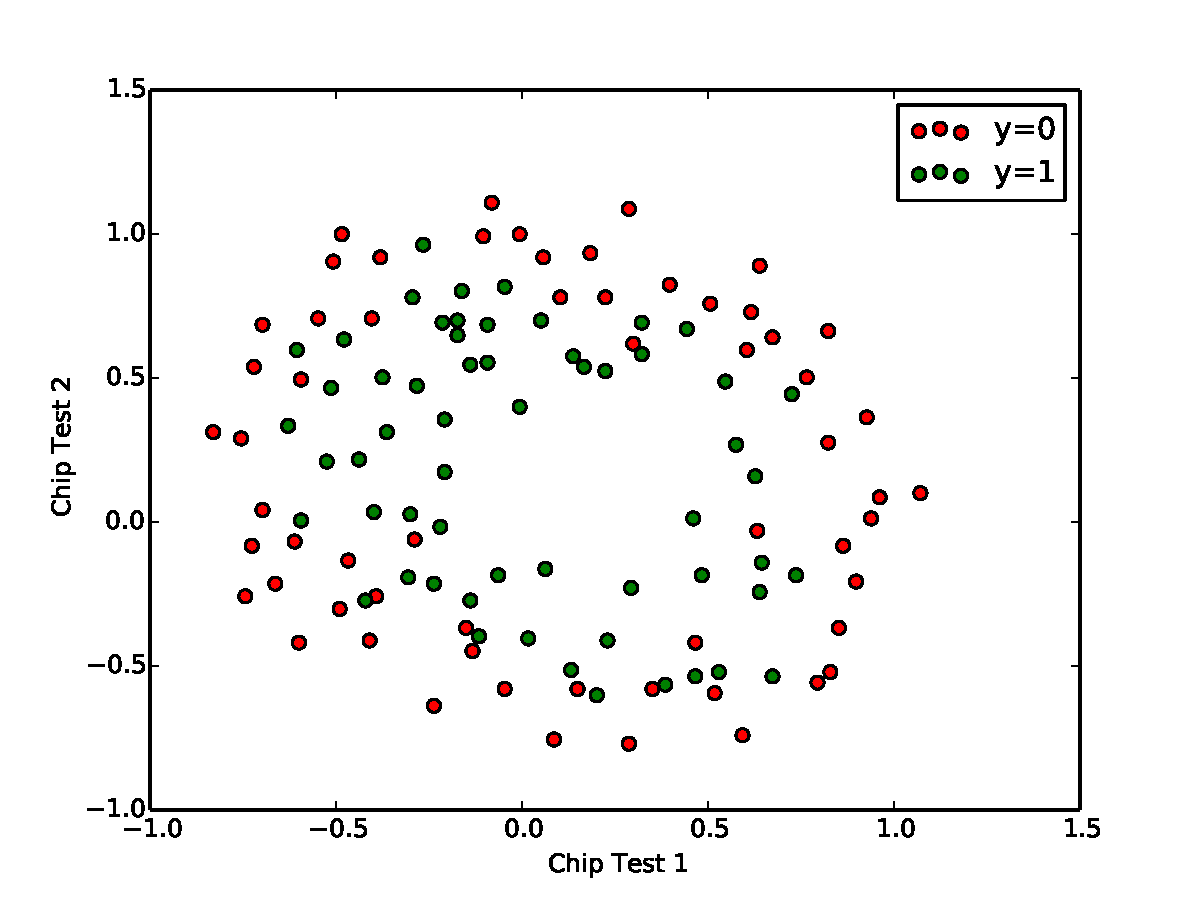
\includegraphics[width=9cm]{part1/fig3.pdf}}}

	

\subcaptionbox{Training data with decision boundary of reg = 1 with sk(l2)}[.5\linewidth]{

	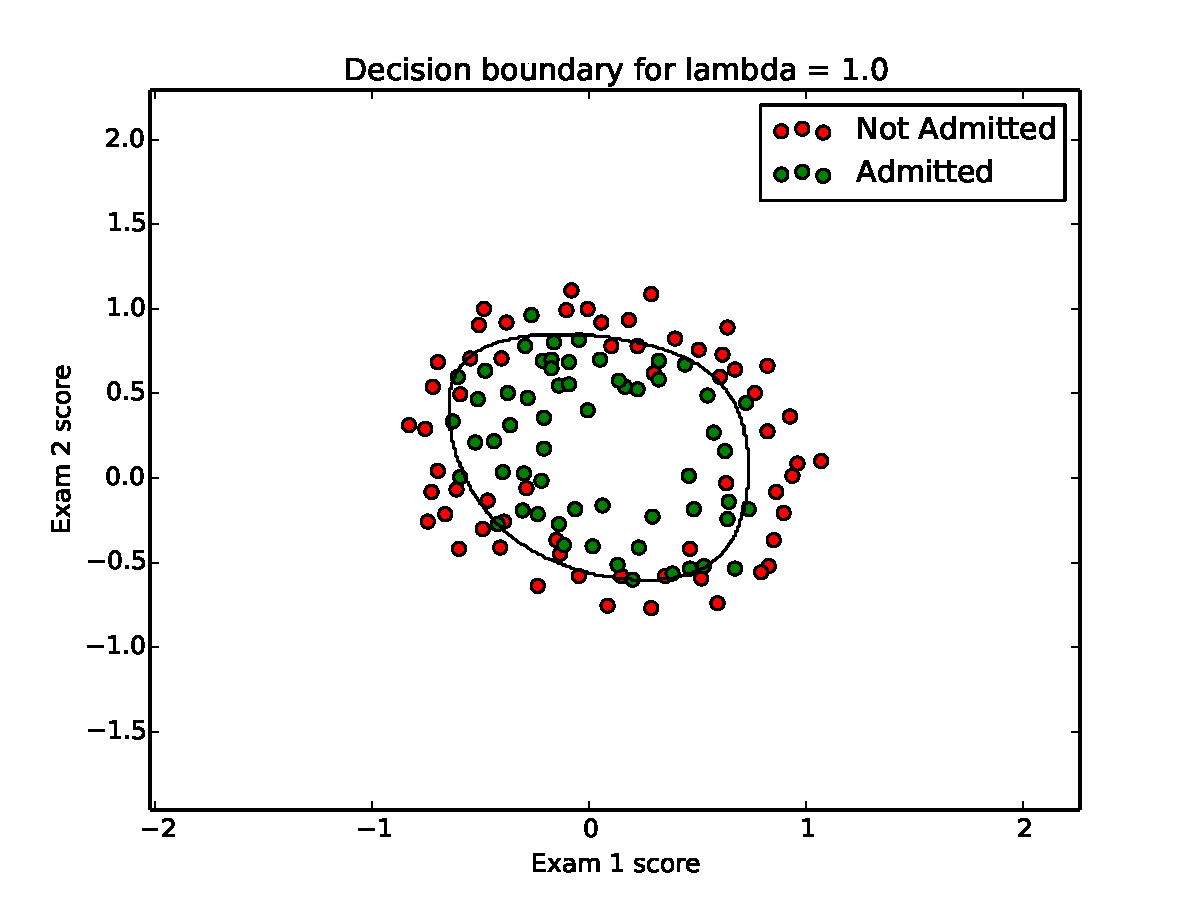
\includegraphics[width=7cm]{part1/fig4_sk.pdf}

	}\subcaptionbox{The regression path of reg = 1}[.5\linewidth]{

	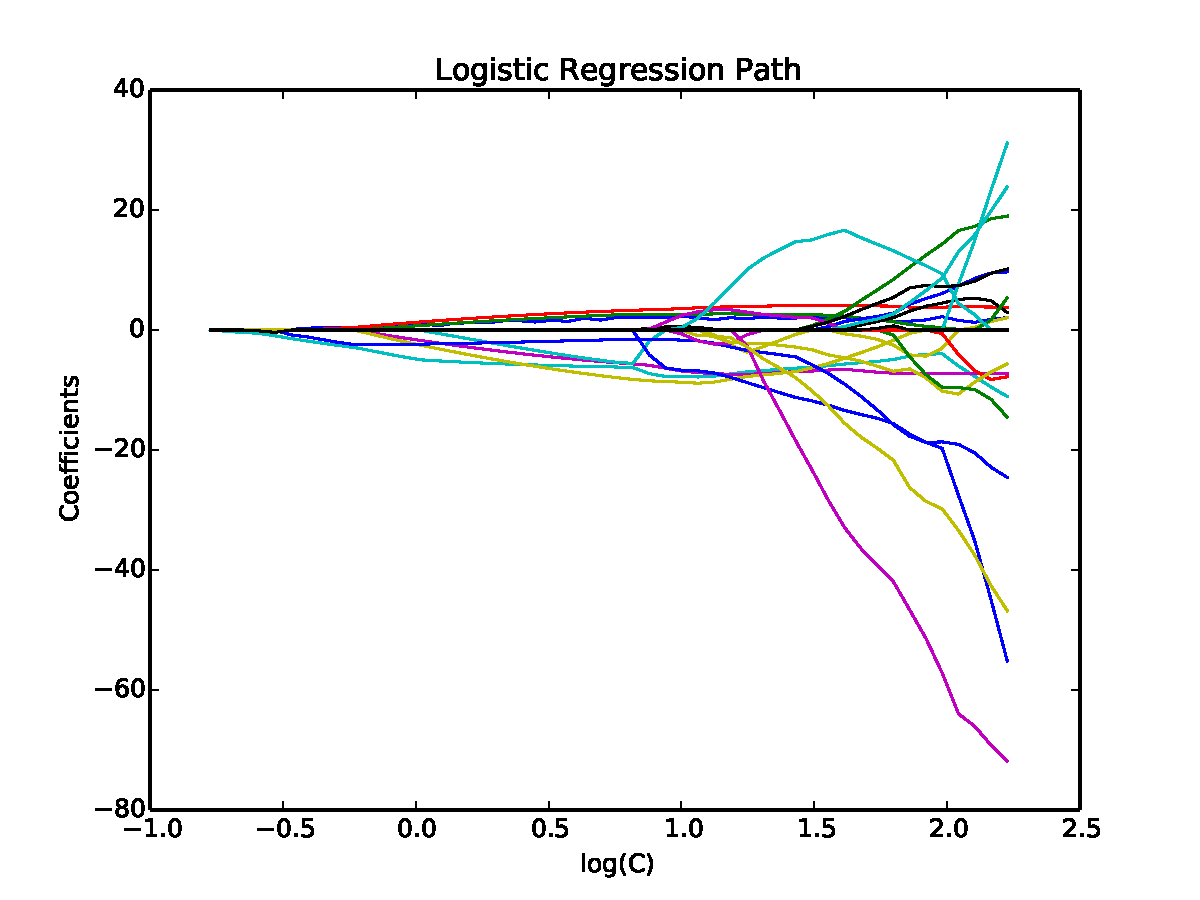
\includegraphics[width=7cm]{part1/fig5.pdf}

	}\caption{}
\end{figure}
\begin{figure}[H]


\centering{\subcaptionbox{Overfitted boundary}{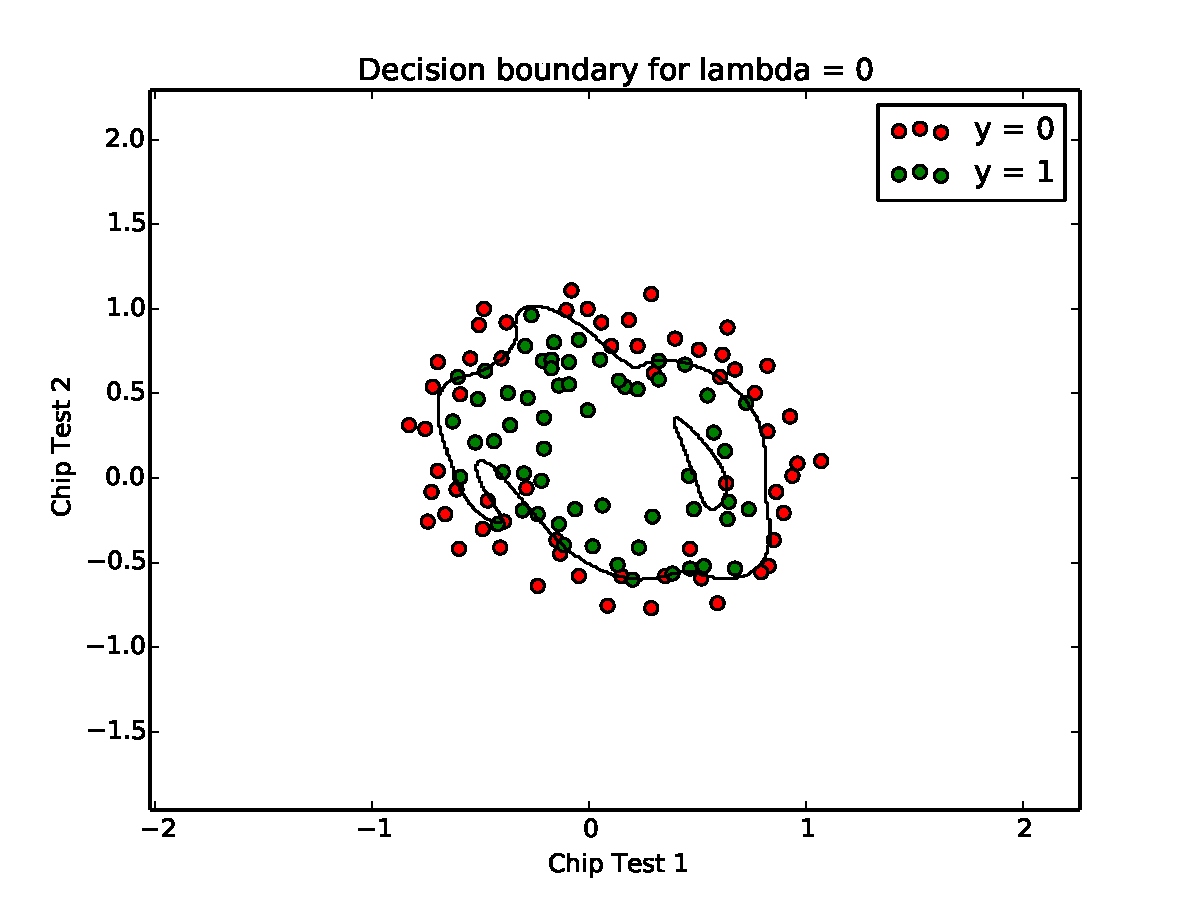
\includegraphics[width=7cm]{part1/fig4_lambda.pdf}}}

	

\subcaptionbox{Properly fitted boundary}[.5\linewidth]{

	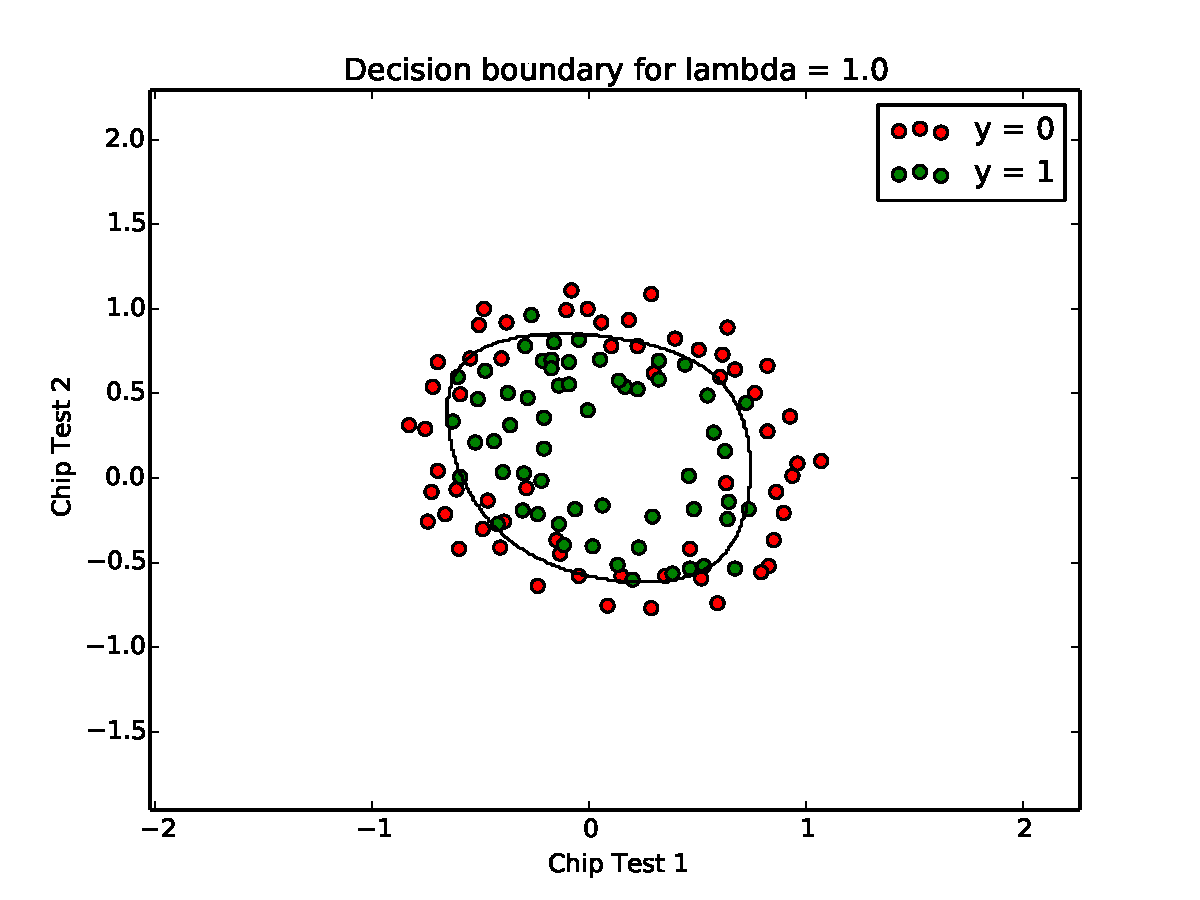
\includegraphics[width=7cm]{part1/fig4_lambda1.pdf}

	}\subcaptionbox{Underfitted boundary}[.5\linewidth]{

	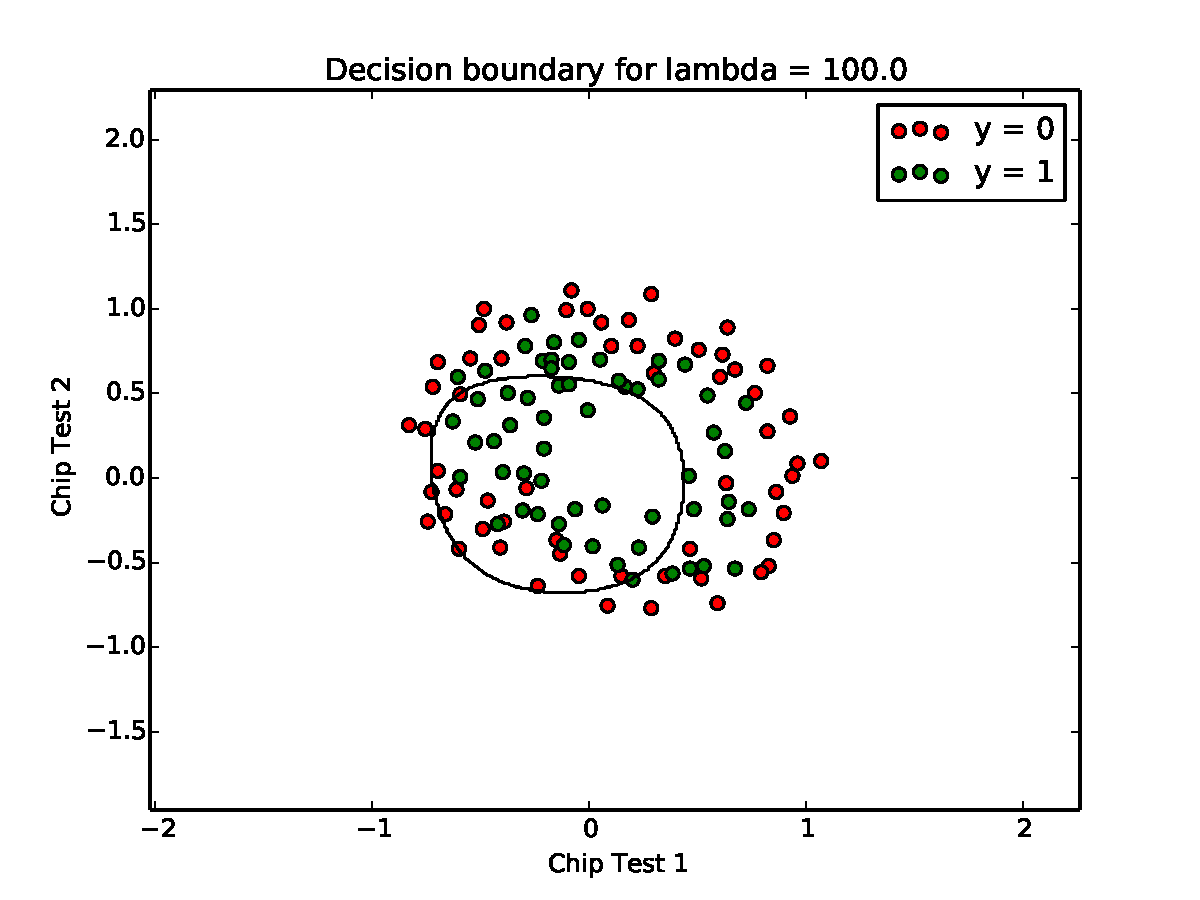
\includegraphics[width=7cm]{part1/fig4_lambda100.pdf}

	}
\caption{Boundary with different reg}

\end{figure}
All as expected. We can see overfitted and underfitted boundary when λ=0 and 100 respectively. \\
When λ increases from 0.1 to 10, the output of l1 reg decreases to 0 more quickly than l2 reg, and the cost of l1 is higher than l2.


\subsection{Part C}

\paragraph{Feature transformation\\}
------\\

Implemented \verb|stdFeatures|, \verb|logTransformFeatures| and \verb|binarizeFeatures| method  in \verb|utils.py|.


\begin{tiny}
\begin{lstlisting}
def log_features(X):
    logf = np.zeros(X.shape)
    # Your code here
    logf = np.log(X+0.1)
    # End your ode
    return logf
def bin_features(X):
    tX = np.zeros(X.shape)
    # your code here
    tX = np.array(X>0,dtype=int)
    # end your code
    return tX
\end{lstlisting}
\end{tiny}

\paragraph{Feature transformation\\}
------\\

Implemented \verb|select_lambda_crossval| method  in \verb|utils.py|.
\begin{tiny}
\begin{lstlisting}
def select_lambda_crossval(X,y,lambda_low,lambda_high,lambda_step,penalty):

    best_lambda = lambda_low

    # Your code here
    # Implement the algorithm above.
    best_accu=0
    kf=cross_validation.KFold(y.shape[0],10)
    l=lambda_low
    while l<=lambda_high:    
        accu=0
        for train_index, test_index in kf:
            xx=X[train_index]
            yy=y[train_index]
            xt=X[test_index]
            yt=y[test_index]
            if penalty == "l2":
                lreg = linear_model.LogisticRegression(penalty=penalty,C=1.0/best_lambda, solver='lbfgs',fit_intercept=True)
            else:
                lreg = linear_model.LogisticRegression(penalty=penalty,C=1.0/best_lambda, solver='liblinear',fit_intercept=True)
            lreg.fit(xx,yy)
            predy = lreg.predict(xt)
            accu=accu+np.mean(predy==yt)
	accu=accu/10
        if accu>best_accu:
            best_accu=accu
            best_lambda=l
        l=l+lambda_step
    # end your code

    return best_lambda

\end{lstlisting}
\end{tiny}
\paragraph{Result\\}
------\\
Run \verb|ex1_spam.py| in the shell:
\begin{tiny}
\begin{lstlisting}
L2 Penalty experiments -----------
best_lambda =  0.1
Coefficients =  [-4.86311314] [[ -2.74144964e-02  -2.25297922e-01   1.21840741e-01   2.29363175e+00
    2.70425757e-01   2.32851060e-01   9.28595406e-01   2.95200115e-01
    1.62205894e-01   6.78255634e-02  -8.32602218e-02  -1.60373332e-01
   -4.72248839e-02   1.07676572e-02   1.87904870e-01   8.19771733e-01
    5.09529185e-01   3.98709124e-02   2.67729599e-01   3.47046562e-01
    2.60498968e-01   3.64607069e-01   7.25020572e-01   1.96728174e-01
   -3.15395736e+00  -4.03134022e-01  -1.25451015e+01  -6.16564148e-02
   -1.56114501e+00  -5.51433441e-02  -3.00843039e-02   4.07264561e-01
   -3.68156729e-01  -1.43612275e+00  -5.87186446e-01   4.44293905e-01
    4.23160725e-02  -1.56897114e-01  -4.55330242e-01  -1.02250011e-01
   -3.54273381e+00  -1.72944271e+00  -4.37530043e-01  -1.05999937e+00
   -9.18599054e-01  -1.75490185e+00  -1.67475688e-01  -9.56877080e-01
   -3.65654247e-01  -1.36535823e-01  -6.58693028e-02   2.06714195e-01
    1.70694494e+00   1.21460221e+00  -3.35271575e-01   1.56142019e+00
    3.68774998e-01]]
Accuracy on set aside test set for  std  =  0.9296875
best_lambda =  0.1
Coefficients =  [-1.40695708] [[-0.1748124  -0.05135689 -0.12339923  1.2828822   0.46456529  0.26013964
   0.96479518  0.48101469  0.11530886  0.15833164 -0.10051294 -0.1852999
  -0.33761946  0.24045718  0.42765064  0.52228884  0.60140119 -0.10265903
   0.12174456  0.29864954  0.20432531  0.18931018  0.54668794  0.56311458
  -1.37213787  0.09174394 -3.52244763  0.25886851 -0.20749972  0.07686118
   0.40469082  1.04149701 -0.15729015  1.29670296 -0.45104347  0.47004354
  -0.35705768  0.36273978 -0.33026736  0.03533685 -0.31829402 -0.93876559
  -0.68715245 -0.80497352 -0.44309598 -0.93099029  0.18540049 -0.84891725
  -0.43476012 -0.12763685  0.19196783  0.7830564   1.47892381  0.02683296
   0.69607044  0.04929847  0.36289482]]
Accuracy on set aside test set for  logt  =  0.943359375
best_lambda =  0.1
Coefficients =  [-1.77183673] [[-0.27016277 -0.13652572 -0.44105224  0.19593277  1.09940287  0.28381492
   2.39371265  0.89847243  0.26535465  0.435632   -0.39728324 -0.42882819
  -1.07464275  0.32304905  0.66670341  1.58604221  1.10348806 -0.17358757
   0.2491685   0.767151    0.78417213  1.4247451   1.03887036  1.61862715
  -2.93738195 -0.23315908 -5.85002477  1.26265761 -0.83080782 -0.06708161
  -1.65512023 -1.71956092 -0.92718438  0.44756264 -0.73938996  0.51818083
  -1.06394957  1.07675048 -0.98242564 -0.32995306 -2.96965659 -2.5398783
  -1.21092653 -2.16550138 -0.85215133 -2.56736788  0.03483552 -2.02741466
  -0.37386944  0.22126778 -0.2152468   1.27339759  1.5956514  -0.03237894
  -0.04463836 -0.04463836 -0.04463836]]
Accuracy on set aside test set for  bin  =  0.92578125
L1 Penalty experiments -----------
best_lambda =  2.1
Coefficients =  [-2.72840332] [[ -1.93809370e-02  -1.90165421e-01   1.26218367e-01   4.56664238e-01
    2.58423508e-01   2.02669188e-01   9.10326804e-01   2.92930859e-01
    1.58447578e-01   5.59232984e-02  -5.60502424e-02  -1.51431784e-01
   -2.86214584e-02   1.08977734e-02   1.74617696e-01   7.93158066e-01
    4.83667987e-01   5.45908763e-02   2.63677888e-01   2.67168004e-01
    2.50977911e-01   3.57024814e-01   7.25613219e-01   2.17779610e-01
   -2.75446443e+00  -3.78683120e-01  -6.94538791e+00  -3.94769408e-02
   -6.47743850e-01  -9.90081163e-03   0.00000000e+00   0.00000000e+00
   -3.58637375e-01   0.00000000e+00  -1.57522300e-01   3.32751667e-01
    4.09903100e-03  -1.34993641e-01  -3.79065669e-01  -6.46707542e-02
   -6.35617521e-01  -1.10564315e+00  -2.72601780e-01  -7.83678731e-01
   -8.24016676e-01  -1.45018868e+00  -1.23169859e-01  -7.13330756e-01
   -3.01341655e-01  -1.31923358e-01  -5.95346647e-02   2.09510366e-01
    1.67669131e+00   5.59770230e-01  -7.64465943e-02   9.25879899e-01
    3.43024768e-01]]
Accuracy on set aside test set for  std  =  0.92578125
best_lambda =  5.1
Coefficients =  [ 0.] [[-0.02237023  0.         -0.05154852  0.16878365  0.42402059  0.15412008
   0.93326218  0.43544729  0.02545247  0.08676809  0.         -0.18887613
  -0.14290738  0.14542169  0.03694076  0.5082957   0.47578605  0.
   0.0795449   0.12335347  0.20266011  0.12228524  0.53917235  0.52854023
  -1.08571406  0.         -1.54138485  0.02033182  0.          0.          0.
   0.         -0.04969466  0.          0.          0.31653286 -0.36289535
   0.         -0.11699187  0.          0.         -0.55663169  0.
  -0.35628821 -0.33859048 -0.77802727  0.         -0.23452883 -0.02391159
   0.          0.          0.75476966  1.30466053  0.          0.55834284
   0.15493247  0.16648669]]
Accuracy on set aside test set for  logt  =  0.940755208333
best_lambda =  0.1
Coefficients =  [-0.23362403] [[-0.27341794 -0.1210642  -0.43824938  0.13312448  1.10360255  0.29869675
   2.42028679  0.90527665  0.26731351  0.44562181 -0.41187711 -0.42707819
  -1.09389899  0.3194352   0.66224276  1.59519397  1.13534114 -0.1819026
   0.24500927  0.80099193  0.78677071  1.41392778  1.03768696  1.65676144
  -3.01060339 -0.19787025 -6.21759202  1.30722175 -0.83095457 -0.04058604
  -1.74016234 -1.90105145 -0.9445934   0.20424823 -0.72605373  0.52532324
  -1.0517627   1.10852783 -0.99529849 -0.30705931 -4.06519585 -2.61231263
  -1.25451571 -2.21821251 -0.8609704  -2.58705802  0.         -2.10652216
  -0.3809371   0.22010838 -0.20768955  1.28165763  1.61412763 -0.0199922
  -0.23270361 -1.0056229  -0.43930022]]
Accuracy on set aside test set for  bin  =  0.92578125

\end{lstlisting}
\end{tiny}

All as expected. \\
We can see that the l1 regularization could exclude unrelated features better. For 3 normalization mathods, the logt method works the best.

\subsection{Part D}
\paragraph{Training one-vs-all logistic regression classifiers\\}
------\\
Implemented \verb|train| method in \verb|one_vs_allLogisticRegressor| class in \verb|one_vs_all.py|.
\begin{tiny}
\begin{lstlisting}
 solver_type = 'NULL'
 if (penalty == 'l2'):
    solver_type = 'lbfgs'
 if (penalty == 'l1'):
    solver_type = 'liblinear'
            
 sk_logreg = linear_model.LogisticRegression(C=1.0/reg,solver=solver_type,fit_intercept=False)
        
 for i in range(0,len(self.labels)):
     sk_logreg.fit(X,1*(y == i))
     theta_opt[i,:] = sk_logreg.coef_[0]
\end{lstlisting}
\end{tiny}

\paragraph{Predicting with a one-vs-all classifier\\}
------\\
Implemented \verb|predict| method in \verb|one_vs_allLogisticRegressor| class in \verb|one_vs_all.py|.
\begin{tiny}
\begin{lstlisting}
 y_pred = np.argmax(utils.sigmoid(X.dot(self.theta.T)),axis=1)
\end{lstlisting}
\end{tiny}
\newpage
Running \verb|ex_music.py| gives output below
\begin{tiny}
\begin{lstlisting}
Confusion matrix using Mel Cepstral represenation
[[13  0  0  0  0  3  3  0  1  4]
 [ 0 20  0  0  0  2  0  0  0  0]
 [ 3  0 10  0  2  2  1  0  0  3]
 [ 1  0  0 10  1  0  1  1  3  0]
 [ 0  0  3  1 10  0  1  2  2  2]
 [ 2  4  0  1  1  5  0  1  1  1]
 [ 0  0  0  0  1  0 14  0  0  1]
 [ 0  0  0  0  0  0  0 21  0  1]
 [ 3  0  2  2  6  1  1  4  8  0]
 [ 2  0  1  5  1  2  1  1  0  1]]
Confusion matrix using FFT represenation
[[10  1  3  2  1  0  2  0  1  3]
 [ 3 20  1  1  0  1  0  0  0  0]
 [ 0  0  3  0  1  0  3  1  3  2]
 [ 0  1  0  4  2  1  0  1  1  3]
 [ 3  0  3  3  3  2  3  0  4  2]
 [ 1  1  5  4  0 11  1  0  1  4]
 [ 1  0  3  4  1  0  5  0  0  3]
 [ 1  0  2  3  1  1  2  6  1  2]
 [ 4  0  2  2  1  0  2  0  3  5]
 [ 0  0  4  3  1  1  0  0  3  7]]
******************** Problem 3D2 ******************** 
--- Overall accuracy with Mel Cepstral representation 0.56
--- Overall accuracy with Fourier representation 0.36
--- Genre =  blues  accuracy with Mel Cepstral representation 0.541666666667
--- Genre =  blues  accuracy with Fourier representation 0.434782608696
--- Genre =  classical  accuracy with Mel Cepstral representation 0.909090909091
--- Genre =  classical  accuracy with Fourier representation 0.769230769231
--- Genre =  country  accuracy with Mel Cepstral representation 0.47619047619
--- Genre =  country  accuracy with Fourier representation 0.230769230769
--- Genre =  disco  accuracy with Mel Cepstral representation 0.588235294118
--- Genre =  disco  accuracy with Fourier representation 0.307692307692
--- Genre =  hiphop  accuracy with Mel Cepstral representation 0.47619047619
--- Genre =  hiphop  accuracy with Fourier representation 0.130434782609
--- Genre =  jazz  accuracy with Mel Cepstral representation 0.3125
--- Genre =  jazz  accuracy with Fourier representation 0.392857142857
--- Genre =  metal  accuracy with Mel Cepstral representation 0.875
--- Genre =  metal  accuracy with Fourier representation 0.294117647059
--- Genre =  pop  accuracy with Mel Cepstral representation 0.954545454545
--- Genre =  pop  accuracy with Fourier representation 0.315789473684
--- Genre =  reggae  accuracy with Mel Cepstral representation 0.296296296296
--- Genre =  reggae  accuracy with Fourier representation 0.157894736842
--- Genre =  rock  accuracy with Mel Cepstral representation 0.0714285714286
--- Genre =  rock  accuracy with Fourier representation 0.368421052632
\end{lstlisting}
\end{tiny}

\begin{itemize}
\item Mel Cepstral representation gives better prediction than FFT representation.
\item Classical genre is easiest to clasify using Mel Cepstral representation.
\item Rock genre is most difficult to classify with Mel Cepstral representation.
\item The accuracy over all genres is not very sensitive to regularization parameter; but some individual genre's (example: rock,metal) are.
\item One approach to improve performance can be using an intrinsic multiclass classifier.
\end{itemize}

\end{document}
